\footnotesize
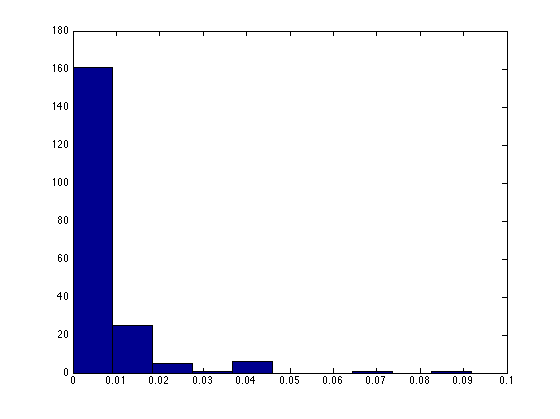
\includegraphics[width=0.3 \linewidth]{./images/Train_features.png}
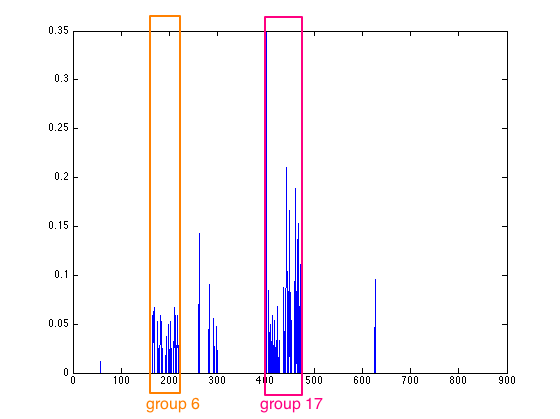
\includegraphics[width=0.3 \linewidth]{./images/mfcc_180.png}
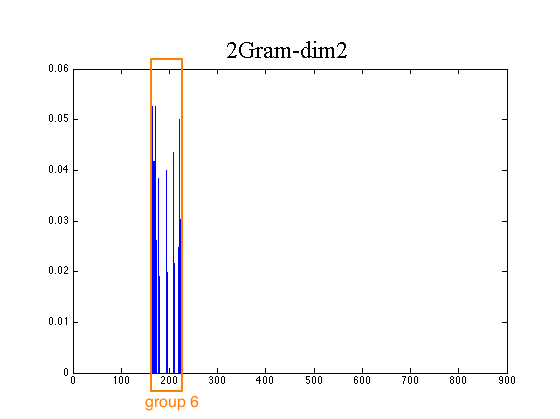
\includegraphics[width=0.32 \linewidth]{./images/ngram_202.png}\\
\footnotesize
Acuuracy of different classifier: \\
The accuarcy for classifier (using Random Forest) on features extracted by the baseline is 0.25. 


\begin{tabular}{cccc}
\multicolumn{1}{c}{\bf Classifier }&\multicolumn{1}{c}{\bf Accuracy}  &\multicolumn{1}{c}{\bf Features} &\multicolumn{1}{c}{\bf Settings}
\\ \hline \\
linear SVM		&67.7273/ 70.4545 		&BoW/ denoised 		&  \\
poly SVM		&69.0909/ 70.4545  	&BoW/ denoised  	& degree: 1  \\
			& 70 			& denoised BoW 	& degree: 2  \\
			& 70.4545  	& denoised BoW 	& degree: 3  \\
rbf SVM       	&70/ 	70.4545  	&BoW/ denoised 		&  \\
                     	&68  			&  BoW (log) 	&  \\
          		&76.8182  		&  denoised BoW 	&  $\gamma = 7.9433$ \\
          		&{\bf 78.1818}  	&  denoised BoW + 2gram 	&    \\
sigmoid SVM     	&70.9091/70.4545	&BoW/ denoised 		&  \\
random forest    	&57/63 			& BoW/ denoised 	& 100 trees; 5 splits \\
       			&63  			& denoised BoW 	& 100 trees; 2 splits \\
NN-euclidean   	&54.09/62.73		& BoW/ denoised 	&  \\
NN-chisquare	&62.27/71.82		& BoW/ denoised 	&  \\

\end{tabular}


